% A filled custom mark shared by the PGFPlots data series and legend.
\documentclass[border=2pt]{standalone}
\usepackage{pgfplots}
\usetikzlibrary{plotmarks}
\pgfplotsset{compat=newest}

\pgfdeclareplotmark{solid caret}{
  \pgfpathmoveto{\pgfqpoint{0pt}{\pgfplotmarksize}}
  \pgfpathlineto{\pgfqpoint{\pgfplotmarksize}{-\pgfplotmarksize}}
  \pgfpathlineto{\pgfqpoint{-\pgfplotmarksize}{-\pgfplotmarksize}}
  \pgfpathclose
  \pgfusepathqfillstroke
}

\begin{document}
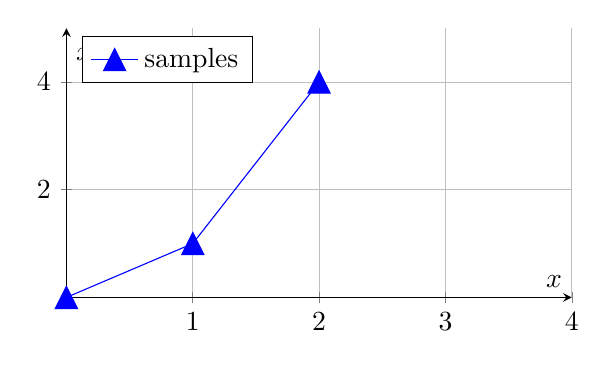
\begin{tikzpicture}
  \begin{axis}[
    width=8cm,height=5cm,
    xmin=0,xmax=4,ymin=0,ymax=5,
    axis lines=middle,grid=major,
    xlabel={$x$},ylabel={$x^2$},
    legend pos=north west
  ]
    \addplot[blue,mark=solid caret,mark size=4pt]
      coordinates {(0,0) (1,1) (2,4)};
    \addlegendentry{samples}
  \end{axis}
\end{tikzpicture}
\end{document}
